% Provenance (never printed): see sources/outline_sources.md (Year 2: fractional
% crystallisation, Bowen's series, compatible and incompatible elements, mixing and
% assimilation, layered intrusions).
% Curves from figdata/bachelor-2/differentiation.py (Bowen 1913 plagioclase loop, Rayleigh and
% equilibrium laws, Wilcox 1954 Paricutin analyses and mass balance, AFC closed form,
% Tegner et al. 2023 Skaergaard whole-rock data); exercise and problem values in the Book 4
% scratch calculator calc/ch08.py.
\chapter{A diferenciação magmática}\label{ch:b2:magmatic-differentiation}

Em 20 de fevereiro de 1943, um vulcão entrou em erupção no oeste do México, e a erupção continuou
durante nove anos. Suas primeiras lavas foram andesitos basálticos com \qty{55}{\percent}
de sílica; as últimas, em fevereiro de 1952, andesitos com pouco mais de
\qty{60}{\percent}. O vulcão, o Parícutin, não mudou de fonte nesse
meio-tempo, e suas lavas foram analisadas uma após a outra à medida que saíam. O
\omterm{def:b2:magma-emplacement:magma}{magma} sob ele mudou por si mesmo: formou cristais e os deixou para trás, e assimilou
parte da rocha granítica ao seu redor. Um \omterm{def:b2:magma-emplacement:magma}{magma} que deixa o manto como basalto pode
terminar como riolito, e as rochas que ele deixa pelo caminho registram como isso aconteceu.
Este capítulo acompanha um \omterm{def:b2:magma-emplacement:magma}{magma} enquanto ele se resfria: a ordem em que os minerais cristalizam,
as leis que dizem como os elementos maiores e os \omterm{def:b2:elements-in-the-earth:trace}{elementos-traço} mudam quando cristais são removidos,
as rochas construídas com esses cristais, e o que acontece quando o \omterm{def:b2:magma-emplacement:magma}{magma} incorpora
outro \omterm{def:b2:magma-emplacement:magma}{magma} ou a crosta.
% ledger: wilcox54:paricutin

\begin{recall}
\textbf{Do volume do ensino médio}: as rochas ígneas e suas texturas; a ordem
em que os minerais cristalizam a partir de um \omterm{def:b2:magma-emplacement:magma}{magma} basáltico, a olivina primeiro e o quartzo por último,
encontrada pelos experimentos de Bowen. \textbf{Do volume do segundo ano dos livros de química}:
os diagramas de fase binários, as soluções sólidas e a regra da alavanca. \textbf{Do volume do primeiro
ano}: o plagioclásio, uma solução sólida entre a anortita \ce{CaAl2Si2O8} e a albita
\ce{NaAlSi3O8}, e os outros silicatos formadores de rochas; as lâminas delgadas entre polarizadores
cruzados. \textbf{Do \cref{ch:b2:elements-in-the-earth}}: os \omterm{def:b2:elements-in-the-earth:partition}{coeficientes de partição mineral--fundido} e
global, $\bar D = \sum_i x_i D_i$, os \omterm{def:b2:elements-in-the-earth:partition}{elementos compatíveis} e incompatíveis,
os \omterm{def:b2:elements-in-the-earth:normalised}{diagramas normalizados} e a \omterm{prop:b2:elements-in-the-earth:normalised}{anomalia de európio}. \textbf{Do
\cref{ch:b2:isotope-geochemistry}}: as razões isotópicas como traçadores e a \omterm{prop:b2:isotope-geochemistry:mixing}{hipérbole
de mistura}. \textbf{Do \cref{ch:b2:mantle-melting}}: o eutético diopsídio--anortita,
a \omterm{def:b2:mantle-melting:peritectic}{fusão incongruente}, os diagramas ternários e os \omterm{def:b2:mantle-melting:primary}{magmas primários}.
\end{recall}

\section{Sequências de cristalização}\label{sec:b2:magmatic-differentiation:sequences}

Um \omterm{def:b2:magma-emplacement:magma}{magma} basáltico não cristaliza todos os seus minerais de uma vez. Bowen verificou
experimentalmente que a olivina normalmente cristaliza primeiro, entre 1200 e
\qty{1300}{\celsius}; que o plagioclásio rico em cálcio começa mais ou menos quando começa o piroxênio;
e que o último líquido, rico em sílica, dá feldspato potássico, quartzo e
talvez muscovita, por volta de 750 a \qty{800}{\celsius}. Entre os dois, os minerais
máficos não simplesmente se acumulam: cada um reage com o líquido para dar o seguinte.
% ledger: earle:bowen (Book 2), tulane:bowen (Book 2)

\begin{definition}[Série de reações de Bowen]\label{def:b2:magmatic-differentiation:bowen}
A \emph{série de reações de Bowen}\index{série de reações de Bowen} é a ordem em que
os silicatos comuns cristalizam a partir de um \omterm{def:b2:magma-emplacement:magma}{magma} basáltico que se resfria, como dois ramos
que se encontram no final. No \emph{ramo descontínuo}, cada mineral máfico
reage com o líquido para formar um novo mineral de outra estrutura: olivina,
piroxênio, anfibólio, biotita. No \emph{ramo contínuo}, o plagioclásio
cristaliza durante todo o processo, com sua composição variando continuamente de rica em cálcio
a rica em sódio. O último líquido cristaliza feldspato potássico, muscovita e
quartzo.
\end{definition}
% ledger: earle:bowen (Book 2)

\begin{omfigure}
\centering
\begin{tikzpicture}[font=\small, x=1cm, y=1cm,
  mn/.style={draw, rounded corners=2pt, fill=white, inner sep=3pt, minimum width=2.3cm,
             align=center}]
\draw[-{Stealth[length=4pt]}, thick, gray] (-1.3,0.3) -- (-1.3,-6.0);
\node[rotate=90, anchor=south, font=\scriptsize, gray] at (-1.4,-2.85) {temperatura decrescente};
\node[anchor=east, font=\scriptsize] at (-1.5,0) {$\approx$ 1200--\qty{1300}{\celsius}};
\node[anchor=east, font=\scriptsize] at (-1.5,-5.6) {$\approx$ 750--\qty{800}{\celsius}};
\node[mn] (ol) at (1,0) {olivina};
\node[mn] (px) at (1,-1.4) {piroxênio};
\node[mn] (am) at (1,-2.8) {anfibólio};
\node[mn] (bt) at (1,-4.2) {biotita};
\draw[-{Stealth[length=4pt]}, thick] (ol) -- (px);
\draw[-{Stealth[length=4pt]}, thick] (px) -- (am);
\draw[-{Stealth[length=4pt]}, thick] (am) -- (bt);
\node[font=\scriptsize, align=center] at (1,0.8) {ramo descontínuo\\(um novo mineral a cada etapa)};
\node[mn] (ca) at (6,-1.4) {plagioclásio\\rico em cálcio};
\node[mn] (na) at (6,-4.2) {plagioclásio\\rico em sódio};
\fill[left color=white, right color=white, top color=orange!35, bottom color=orange!8]
  (5.75,-2.0) rectangle (6.25,-3.6);
\draw[-{Stealth[length=4pt]}, thick] (ca) -- (na);
\node[font=\scriptsize, align=center] at (6,0.8) {ramo contínuo\\(um só mineral, de composição variável)};
\node[mn, minimum width=7.2cm] (last) at (3.5,-5.6) {feldspato potássico, muscovita, quartzo};
\draw[-{Stealth[length=4pt]}, thick] (bt) -- (bt|-last.north);
\draw[-{Stealth[length=4pt]}, thick] (na) -- (na|-last.north);
\end{tikzpicture}
\par\smallskip{\small A \omterm{def:b2:magmatic-differentiation:bowen}{série de reações de Bowen}. A olivina e o plagioclásio rico em cálcio
cristalizam primeiro a partir de um \omterm{def:b2:magma-emplacement:magma}{magma} basáltico; à esquerda, cada mineral máfico reage com
o líquido para dar o seguinte; à direita, o plagioclásio fica cada vez mais rico em
sódio; o último líquido, rico em sílica, dá feldspato potássico, muscovita e quartzo.
As temperaturas são valores típicos para um \omterm{def:b2:magma-emplacement:magma}{magma} basáltico a baixa pressão.}
\end{omfigure}
% ledger: earle:bowen (Book 2)

Os dois ramos correspondem aos dois tipos de diagrama de fase do
\cref{ch:b2:mantle-melting}. Uma reação descontínua é a \omterm{def:b2:mantle-melting:peritectic}{fusão incongruente} da
enstatita percorrida ao contrário: cristais de forsterita reagem com um líquido mais rico em sílica para
dar enstatita. O ramo contínuo é uma solução sólida. Bowen a mediu em 1913
em plagioclásios sintéticos, mantendo cada composição a uma temperatura conhecida e
procurando vidro e cristais: a anortita funde a \qty{1550}{\celsius}, a albita a
cerca de \qty{1100}{\celsius}, e todo plagioclásio intermediário funde em um intervalo
entre uma curva inferior, o solidus, e uma superior, o liquidus (a figura
abaixo).
% ledger: bowen13:plagioclase, bowen14:mgo-sio2

\begin{omfigure}
\centering
\begin{tikzpicture}
\begin{axis}[omrecord, width=0.78\linewidth, height=6.4cm,
  xmin=0, xmax=100, ymin=1050, ymax=1600,
  xlabel={anortita (\unit{\percent}, molar)}, ylabel={temperatura (\unit{\celsius})},
  y tick label style={/pgf/number format/1000 sep={}}, unbounded coords=discard,
  tick label style={font=\scriptsize}, label style={font=\small}]
\addplot[very thick, black] table[x=an, y=T_liq] {figdata/out/bachelor-2-differentiation-plag-curve.dat};
\addplot[very thick, black, dashed] table[x=an, y=T_sol] {figdata/out/bachelor-2-differentiation-plag-curve.dat};
\addplot[only marks, mark=*, mark size=1.5pt, blue!70!black] table[x=an, y=T_liq] {figdata/out/bachelor-2-differentiation-plag-data.dat};
\addplot[only marks, mark=o, mark size=1.7pt, blue!70!black] table[x=an, y=T_sol] {figdata/out/bachelor-2-differentiation-plag-data.dat};
\draw[densely dotted, red!70!black, thick] (axis cs:50,1560) -- (axis cs:50,1287);
\draw[red!70!black, thick] (axis cs:50,1450) -- (axis cs:80.6,1450);
\draw[red!70!black, thick] (axis cs:33.3,1394) -- (axis cs:70.6,1394);
\draw[red!70!black, thick] (axis cs:13.9,1287) -- (axis cs:50,1287);
\addplot[only marks, mark=*, mark size=1.4pt, red!70!black] coordinates {(50,1450) (80.6,1450) (33.3,1394) (70.6,1394) (13.9,1287) (50,1287)};
\node[font=\scriptsize] at (axis cs:30,1530) {líquido};
\node[font=\scriptsize, align=center] at (axis cs:83,1200) {plagioclásio\\(solução sólida)};
\node[font=\scriptsize, anchor=west] at (axis cs:2,1430) {liquidus (linha cheia)};
\node[font=\scriptsize, anchor=west] at (axis cs:42,1160) {solidus (tracejado)};
\node[font=\scriptsize, anchor=south, red!70!black, fill=white, inner sep=1pt] at (axis cs:68,1452) {\qty{1450}{\celsius}};
\node[font=\scriptsize, anchor=north, red!70!black, fill=white, inner sep=1pt] at (axis cs:31,1284) {\qty{1287}{\celsius}};
\end{axis}
\end{tikzpicture}
\par\smallskip{\small Os feldspatos plagioclásios à pressão atmosférica, segundo os
experimentos de têmpera de Bowen (1913): início (círculos) e fim (pontos) da
fusão, com curvas traçadas pelas medidas. Em vermelho, a \omterm{def:b2:magmatic-differentiation:crystallisation}{cristalização em
equilíbrio} de um líquido com \qty{50}{\percent} de anortita: o primeiro cristal, a
\qty{1450}{\celsius}, tem \qty{81}{\percent} de anortita; a \qty{1394}{\celsius},
cristais com \qty{71}{\percent} coexistem com um líquido com \qty{33}{\percent}; o último
líquido, a \qty{1287}{\celsius}, tem \qty{14}{\percent} (\cref{exo:b2:magmatic-differentiation:1}).}
\end{omfigure}
% ledger: bowen13:plagioclase

Um líquido que cristaliza uma solução sólida se enriquece no componente que
funde à temperatura mais baixa: o primeiro plagioclásio de um líquido com
\qty{50}{\percent} de anortita tem \qty{81}{\percent}, e o líquido se desloca em direção à
albita. O que acontece em seguida depende de os cristais continuarem ou não a dialogar com o
líquido.

\begin{definition}[Cristalização em equilíbrio e cristalização fracionada]
\label{def:b2:magmatic-differentiation:crystallisation}
Na \emph{cristalização em equilíbrio}\index{cristalização em equilíbrio}, os
cristais permanecem em equilíbrio químico com a totalidade do líquido até o
fim, reequilibrando-se à medida que o líquido muda; o sistema termina com a composição
com que começou. Na \emph{cristalização fracionada}\index{cristalização fracionada},
cada cristal, uma vez formado, é retirado da reação com o
líquido, por decantação, por ser colado às paredes da câmara ou por ser
encapsulado por um crescimento posterior; o líquido evolui então como se os cristais tivessem
sido retirados do sistema.
\end{definition}

Na \omterm{def:b2:magmatic-differentiation:crystallisation}{cristalização em equilíbrio}, o plagioclásio da figura acima passa de
\qty{81}{\percent} a \qty{50}{\percent} de anortita à medida que cresce, cada cristal
se reequilibrando por difusão com o líquido, e o último líquido desaparece no
solidus, a \qty{1287}{\celsius}. A difusão no feldspato é lenta, e os cristais naturais
raramente acompanham: o interior de cada cristal fica isolado do líquido,
que então se comporta como na \omterm{def:b2:magmatic-differentiation:crystallisation}{cristalização fracionada} e pode chegar a composições
próximas da albita. A figura da última seção deste capítulo calcula os dois caminhos.
% ledger: bowen13:plagioclase

\begin{definition}[Linha de descida do líquido]\label{def:b2:magmatic-differentiation:lld}
A \emph{linha de descida do líquido}\index{linha de descida do líquido} de um \omterm{def:b2:magma-emplacement:magma}{magma} é a
sequência das composições assumidas por seu líquido à medida que ele cristaliza, lançada em um
diagrama de variação ou em um diagrama de fase.
\end{definition}

Uma \omterm{def:b2:magmatic-differentiation:lld}{linha de descida do líquido} é uma propriedade apenas do líquido. As lavas emitidas com
cristais não ficam exatamente sobre ela, e Wilcox, estudando as lavas do
Parícutin, usou tanto suas análises de rocha total quanto as composições de sua
matriz, a parte líquida, calculadas removendo-se os cristais.
% ledger: wilcox54:groundmass

\section{Cristalização fracionada dos elementos maiores}\label{sec:b2:magmatic-differentiation:majors}

Remover cristais altera a composição do líquido de maneira simples e linear,
e a ferramenta mais antiga para lê-la é um gráfico de cada óxido em função da sílica.

\begin{definition}[Diagrama de Harker]\label{def:b2:magmatic-differentiation:harker}
Um \emph{diagrama de Harker}\index{diagrama de Harker} (diagrama de variação em sílica) lança a
porcentagem em massa de cada óxido de uma suíte de rochas aparentadas em função de sua
porcentagem em massa de \ce{SiO2}, um painel por óxido.
\end{definition}


As lavas do Parícutin mostram tais tendências (os \omterm{def:b2:magmatic-differentiation:harker}{diagramas de Harker} depois da próxima
proposição): à medida que a sílica aumenta, a magnésia, a cal e a alumina diminuem e a potassa aumenta. É
o que faria a remoção de olivina e de plagioclásio:
a olivina retira magnésia e ferro, o plagioclásio cal e alumina, e ambos deixam
o líquido mais rico em sílica e em álcalis. Saber se a remoção de minerais conhecidos pode
explicar quantitativamente as tendências é uma questão de balanço de massa.

\begin{proposition}[Balanço de massa da remoção de cristais]\label{prop:b2:magmatic-differentiation:lever}
Suponha-se que um \omterm{def:b2:magma-emplacement:magma}{magma} parental de composição $\mathbf p$ (um vetor de frações em massa de óxidos) cristalize
minerais de composições $\mathbf m_1, \dots, \mathbf m_k$ em massas
$x_1, \dots, x_k$ por unidade de massa de \omterm{def:b2:magma-emplacement:magma}{magma} parental, e seja $\mathbf d$ a composição
do líquido restante. Então
\[
\mathbf p = \Big(1 - \sum_i x_i\Big)\mathbf d + \sum_i x_i \mathbf m_i .
\]
Para um único mineral, o \omterm{def:b2:magma-emplacement:magma}{magma} parental fica sobre o segmento de reta que une o líquido e o
mineral em todo diagrama de variação, e a fração em massa removida é
$x = (p_j - d_j)/(m_j - d_j)$ para qualquer óxido $j$: a regra da alavanca.
\end{proposition}

\begin{proof}
Todo óxido se conserva: a massa $p_j$ do óxido $j$ em uma unidade de massa de \omterm{def:b2:magma-emplacement:magma}{magma} parental termina
ou no líquido, de massa $1 - \sum_i x_i$ e concentração $d_j$, ou nos
minerais. Escrever isso para cada $j$ dá a equação vetorial. Com um único mineral, ela
se escreve $\mathbf p = (1-x)\mathbf d + x\mathbf m$, um ponto do segmento de
$\mathbf d$ a $\mathbf m$ que o divide na razão $x : (1-x)$, em qualquer par de
eixos; resolver uma componente dá $x$.
\end{proof}

\begin{omfigure}
\centering
\begin{tikzpicture}
\begin{groupplot}[group style={group size=2 by 2, horizontal sep=1.6cm, vertical sep=1.3cm},
  width=0.44\linewidth, height=4.3cm, omrecord, xmin=54.5, xmax=60.8,
  tick label style={font=\scriptsize}, label style={font=\small},
  xtick={55,56,57,58,59,60}]
\nextgroupplot[ylabel={\ce{MgO} (\unit{\percent})}, ymin=3.2, ymax=6.0]
\addplot[only marks, mark=*, mark size=1.3pt, blue!70!black] table[x=SiO2, y=MgO] {figdata/out/bachelor-2-differentiation-paricutin.dat};
\nextgroupplot[ylabel={\ce{CaO} (\unit{\percent})}, ymin=6.0, ymax=7.6]
\addplot[only marks, mark=*, mark size=1.3pt, blue!70!black] table[x=SiO2, y=CaO] {figdata/out/bachelor-2-differentiation-paricutin.dat};
\nextgroupplot[ylabel={\ce{K2O} (\unit{\percent})}, ymin=0.7, ymax=1.9, xlabel={\ce{SiO2} (\unit{\percent})}]
\addplot[only marks, mark=*, mark size=1.3pt, blue!70!black] table[x=SiO2, y=K2O] {figdata/out/bachelor-2-differentiation-paricutin.dat};
\node[font=\scriptsize, anchor=west] at (axis cs:55.1,0.80) {1943};
\node[font=\scriptsize, anchor=east] at (axis cs:60.0,1.82) {1952};
\nextgroupplot[ylabel={\ce{Al2O3} (\unit{\percent})}, ymin=17.0, ymax=19.0, xlabel={\ce{SiO2} (\unit{\percent})}]
\addplot[only marks, mark=*, mark size=1.3pt, blue!70!black] table[x=SiO2, y=Al2O3] {figdata/out/bachelor-2-differentiation-paricutin.dat};
\end{groupplot}
\end{tikzpicture}
\par\smallskip{\small \omterm{def:b2:magmatic-differentiation:harker}{Diagramas de Harker} das 22 lavas do Parícutin analisadas por
Wilcox (1954), emitidas de fevereiro de 1943 (sílica mais baixa) a fevereiro de 1952. À medida que
a sílica aumenta cinco por cento, a magnésia, a cal e a alumina diminuem e a potassa quase
dobra.}
\end{omfigure}
% ledger: wilcox54:table2, wilcox54:paricutin

Com vários minerais, as massas são encontradas resolvendo as equações de conservação de
outros tantos óxidos. Wilcox fez isso graficamente em 1954; hoje é um pequeno sistema
linear.

\begin{method}[Balanço de massa por mínimos quadrados]\label{met:b2:magmatic-differentiation:massbalance}
Para testar se um líquido derivado $\mathbf d$ provém de um \omterm{def:b2:magma-emplacement:magma}{magma} parental $\mathbf p$ pela
remoção dos minerais $\mathbf m_1, \dots, \mathbf m_k$ (e pela adição, se necessário, de uma
rocha assimilada, introduzida com massa negativa): (1) para cada óxido $j$, escreva-se a
conservação da proposição reorganizada como uma equação linear nas massas
removidas por \qty{100}{g} de \omterm{def:b2:magma-emplacement:magma}{magma} parental,
\[
\sum_i x_i\,(m_{ij} - d_j) = 100\,(p_j - d_j);
\]
(2) com exatamente $k$ óxidos, escolhidos entre os que os minerais mais alteram, resolva-se o
sistema $k \times k$; com mais óxidos, resolva-se por mínimos quadrados (minimizando a soma
dos quadrados das diferenças entre os dois membros); (3) recalcule-se o líquido derivado a partir
das massas encontradas e compare-se com a análise, óxido por óxido: resíduos maiores
que os erros analíticos, ou uma massa negativa para um mineral, rejeitam o modelo.
\end{method}

Wilcox escolheu a sílica, a alumina e a magnésia como seus três controles, e três
materiais: olivina de composição Fo$_{80}$, plagioclásio An$_{70}$ e a média
de quatro xenólitos graníticos (\qty{72.5}{\percent} de \ce{SiO2}, \qty{3.6}{\percent} de
\ce{K2O}) encontrados nas lavas. Ele mostrou que nenhuma combinação de olivina e
plagioclásio sozinhos se ajusta à série, e que acrescentar \qty{25.4}{g} de xenólito e
remover \qty{2.9}{g} de olivina e \qty{9.6}{g} de plagioclásio de
\qty{100}{g} da matriz da primeira lava dá \qty{112.9}{g} de um material
próximo da matriz da lava de 1950. Resolver exatamente suas três equações
dá \qty{24.6}{g}, \qty{3.1}{g} e \qty{9.9}{g}; os mínimos quadrados sobre sete óxidos
dão uma resposta diferente, \qty{28.7}{g}, \qty{2.4}{g} e \qty{5.7}{g}, o que lembra
que tais resultados dependem dos controles escolhidos. De um modo ou de outro, o \omterm{def:b2:magma-emplacement:magma}{magma} incorporou mais
granito do que cristalizou. As lavas do Parícutin registram um sistema aberto, o
assunto da última seção.
% ledger: wilcox54:mass-balance, wilcox54:xenoliths, wilcox54:groundmass

\section{Os elementos-traço}\label{sec:b2:magmatic-differentiation:trace}

Um \omterm{def:b2:elements-in-the-earth:trace}{elemento-traço} não altera os minerais que cristalizam; ele os acompanha,
com seu coeficiente de partição global $\bar D$ (\cref{ch:b2:elements-in-the-earth}),
aqui escrito $D$, entre os cristais que se formam a cada momento e o líquido.

\begin{theorem}[Lei de fracionamento de Rayleigh]\label{thm:b2:magmatic-differentiation:rayleigh}
Na \omterm{def:b2:magmatic-differentiation:crystallisation}{cristalização fracionada} perfeita com um coeficiente de partição global constante
$D$, a concentração de um \omterm{def:b2:elements-in-the-earth:trace}{elemento-traço} no líquido é
\[
\frac{C_L}{C_0} = F^{\,D-1},
\]
onde $C_0$ é sua concentração no líquido inicial e $F$ a fração em massa de
líquido restante.
Esta é a \emph{lei de fracionamento de Rayleigh}\index{lei de fracionamento de Rayleigh}.
\end{theorem}

\begin{proof}
Seja $M$ a massa de líquido. Quando uma pequena massa $-\mathrm dM > 0$ de cristais
se forma, em equilíbrio com o líquido apenas naquele momento, ela leva o elemento à
concentração $DC_L$. A massa do elemento no líquido, $MC_L$, varia portanto
de $\mathrm d(MC_L) = DC_L\,\mathrm dM$. Desenvolvendo, $M\,\mathrm dC_L = (D-1)C_L\,
\mathrm dM$, logo $\mathrm dC_L/C_L = (D-1)\,\mathrm dM/M$. Integrar a partir de $M_0$,
onde $C_L = C_0$, dá $\ln(C_L/C_0) = (D-1)\ln(M/M_0)$, e $F = M/M_0$.
\end{proof}

\begin{proposition}[Cristalização em equilíbrio de um elemento-traço]
\label{prop:b2:magmatic-differentiation:equilibrium}
Se os cristais permanecem em equilíbrio com o líquido, $C_L/C_0 = 1/(D + F(1-D))$.
\end{proposition}

\begin{proof}
Toda a massa cristalina $1-F$ (por unidade de massa inicial) contém $DC_L$, de modo que a conservação
da massa do elemento se escreve $C_0 = FC_L + (1-F)DC_L$.
\end{proof}

\begin{corollary}[Razões de elementos incompatíveis]\label{cor:b2:magmatic-differentiation:ratio}
Para dois elementos de coeficientes de partição $D_1$ e $D_2$, a razão entre suas
concentrações no líquido muda pelo fator $F^{\,D_1-D_2}$ na \omterm{def:b2:magmatic-differentiation:crystallisation}{cristalização
fracionada}. Se ambos são fortemente incompatíveis ($D_1, D_2 \ll 1$), a razão
quase não muda: conserva o valor do \omterm{def:b2:magma-emplacement:magma}{magma} parental, e portanto de sua fonte.
\end{corollary}

\begin{proof}
Dividam-se as duas leis de Rayleigh: $(C_1/C_2)/(C_{1,0}/C_{2,0}) = F^{D_1-1}/F^{D_2-1}$;
para $F = 0.5$ e $D_1 - D_2 = 0.05$, o fator é $0.5^{0.05} = 0.97$.
\end{proof}

\begin{omfigure}
\centering
\begin{tikzpicture}
\begin{axis}[omrecord, width=0.78\linewidth, height=6.4cm, ymode=log,
  xmin=0, xmax=1, ymin=0.01, ymax=100, x dir=reverse,
  xlabel={fração de líquido restante $F$}, ylabel={$C_L/C_0$},
  legend columns=3, legend style={font=\scriptsize, at={(0.02,0.97)}, anchor=north west},
  tick label style={font=\scriptsize}, label style={font=\small}]
\addplot[thick, red!75!black] table[x=F, y=d0.01] {figdata/out/bachelor-2-differentiation-rayleigh.dat};
\addlegendentry{$D = 0.01$}
\addplot[thick, orange!80!black] table[x=F, y=d0.1] {figdata/out/bachelor-2-differentiation-rayleigh.dat};
\addlegendentry{0.1}
\addplot[thick, olive] table[x=F, y=d0.5] {figdata/out/bachelor-2-differentiation-rayleigh.dat};
\addlegendentry{0.5}
\addplot[thick, teal] table[x=F, y=d2] {figdata/out/bachelor-2-differentiation-rayleigh.dat};
\addlegendentry{2}
\addplot[thick, blue!70!black] table[x=F, y=d5] {figdata/out/bachelor-2-differentiation-rayleigh.dat};
\addlegendentry{5}
\addplot[thick, violet] table[x=F, y=d10] {figdata/out/bachelor-2-differentiation-rayleigh.dat};
\addlegendentry{10}
\addplot[thick, dashed, forget plot, red!75!black] table[x=F, y=e0.01] {figdata/out/bachelor-2-differentiation-rayleigh.dat};
\addplot[thick, dashed, forget plot, orange!80!black] table[x=F, y=e0.1] {figdata/out/bachelor-2-differentiation-rayleigh.dat};
\addplot[thick, dashed, forget plot, teal] table[x=F, y=e2] {figdata/out/bachelor-2-differentiation-rayleigh.dat};
\addplot[thick, dashed, forget plot, violet] table[x=F, y=e10] {figdata/out/bachelor-2-differentiation-rayleigh.dat};
\end{axis}
\end{tikzpicture}
\par\smallskip{\small Concentração de um \omterm{def:b2:elements-in-the-earth:trace}{elemento-traço} no líquido em função da
fração de líquido restante, para coeficientes de partição globais de 0.01 a 10:
\omterm{def:b2:magmatic-differentiation:crystallisation}{cristalização fracionada} (linhas cheias, lei de Rayleigh) e \omterm{def:b2:magmatic-differentiation:crystallisation}{cristalização em
equilíbrio} (tracejadas, para $D = 0.01$, 0.1, 2 e 10). Os \omterm{def:b2:elements-in-the-earth:partition}{elementos incompatíveis} aumentam no máximo como $1/F$;
os \omterm{def:b2:elements-in-the-earth:partition}{elementos compatíveis} despencam, tanto mais depressa quanto maior for $D$, e a \omterm{def:b2:magmatic-differentiation:crystallisation}{cristalização
fracionada} os remove quase completamente.}
\end{omfigure}

A figura acima se lê em dois sentidos. Os \omterm{def:b2:elements-in-the-earth:partition}{elementos incompatíveis} ($D \ll 1$) se comportam
quase da mesma forma: sua concentração aumenta quase como $1/F$, de modo que um líquido enriquecido
dez vezes em zircônio cristalizou cerca de nove décimos de sua massa. Os \omterm{def:b2:elements-in-the-earth:partition}{elementos compatíveis}
são muito mais sensíveis. O níquel entra na olivina com um coeficiente de partição
de cerca de 5 nos líquidos magnesianos quentes: medido em 3.8 a
\qty{1550}{\celsius} e em 5.0 a \qty{1400}{\celsius}, ele aumenta cerca de 0.8 a cada
\qty{100}{\celsius} de resfriamento; o estrôncio entra no
plagioclásio com cerca de 2.7; um basalto que cristaliza um quinto de sua massa como
olivina perde mais da metade de seu níquel (\cref{exo:b2:magmatic-differentiation:5}). O níquel é portanto o
registro mais sensível do fracionamento da olivina, e um basalto rico em níquel está
próximo de um \omterm{def:b2:mantle-melting:primary}{magma primário} (\cref{ch:b2:mantle-melting}).
% ledger: matzen12:dni, white07:kd-basalt

Duas observações fixam o alcance dessas leis. Primeiro, $D$ não é uma constante: ele muda
quando um novo mineral se junta à assembleia que cristaliza, e a lei é então aplicada
por etapas (\cref{exo:b2:magmatic-differentiation:12}). Segundo, as mesmas equações, com os papéis do sólido e do
líquido trocados, descrevem a fusão de uma fonte; como a fusão em lote e a fusão fracionada
fracionam os \omterm{def:b2:elements-in-the-earth:trace}{elementos-traço} é tratado no volume do terceiro ano.

\section{Cumulatos e intrusões acamadas}\label{sec:b2:magmatic-differentiation:cumulates}

Para onde vão os cristais removidos de um \omterm{def:b2:magma-emplacement:magma}{magma}? Em uma câmara magmática que se resfria
lentamente, eles decantam em seu assoalho, crescem em suas paredes e em seu teto, e constroem rochas de um
tipo particular.

\begin{definition}[Cumulato; intrusão acamada]\label{def:b2:magmatic-differentiation:cumulate}
Um \emph{cumulato}\index{cumulato} é uma rocha ígnea formada pela acumulação de
cristais (os cristais cúmulus) a partir de um \omterm{def:b2:magma-emplacement:magma}{magma}, junto com os minerais que cresceram depois
a partir do líquido aprisionado entre eles (o material intercúmulus); sua composição
é a de cristais mais um pouco de líquido, e não a de um \omterm{def:b2:magma-emplacement:magma}{magma}. Uma \emph{intrusão
acamada}\index{intrusão acamada} é um grande corpo, resfriado lentamente, de cumulatos máficos ou
ultramáficos dispostos em camadas, que registra a \omterm{def:b2:magmatic-differentiation:crystallisation}{cristalização fracionada} do
\omterm{def:b2:magma-emplacement:magma}{magma} que o preencheu.
\end{definition}

A intrusão de Skaergaard, no leste da Groenlândia, com cerca de \qty{56}{Ma}, é a
referência. Seus gabros acamados afloram em cerca de 11 por \qty{8}{km}, e registram a
diferenciação ininterrupta de um basalto toleítico: uma Série Acamada cresceu no
assoalho, uma Série Marginal nas paredes e no teto, e as duas se encontraram no Horizonte Sanduíche,
onde o último líquido, o mais evoluído, cristalizou no interior (a figura abaixo).
Os \omterm{def:b2:magmatic-differentiation:cumulate}{cumulatos} do assoalho são divididos, da base para o topo, em uma Zona Oculta, não exposta,
e nas Zonas Inferior, Média e Superior, expostas. Seus
estudiosos estimaram a fração em massa $F$ de líquido restante quando cada nível cristalizou, ajustada
ao longo da seção de referência da Série Acamada por
\[
F = \num{1.091e-7}\,H^2 - \num{5.9064e-4}\,H + 0.7678
\]
($H$ em metros acima da base da Zona Inferior). Um quarto do \omterm{def:b2:magma-emplacement:magma}{magma} já tinha
cristalizado, nas paredes, no teto e em uma zona oculta, quando a sequência exposta do
assoalho começou; o Horizonte Sanduíche, $F = 0$, fica uns \qty{2.2}{km} acima
(\cref{exo:b2:magmatic-differentiation:7}).
% ledger: tegner23:skaergaard

\begin{omfigure}
\centering
\begin{tikzpicture}[x=1cm, y=1cm, font=\scriptsize]
\fill[gray!20] (-5.4,-0.5) rectangle (5.4,4.9);
\node[anchor=south west] at (-5.35,4.35) {rocha encaixante};
\fill[orange!35] (-4.6,0) rectangle (4.6,1.1);
\fill[orange!22] (-4.2,1.1) rectangle (4.2,1.9);
\fill[orange!12] (-3.8,1.9) rectangle (3.8,2.55);
\fill[blue!12] (-4.6,4.3) rectangle (4.6,3.75);
\fill[blue!20] (-4.2,3.75) rectangle (4.2,3.25);
\fill[blue!28] (-3.8,3.25) rectangle (3.8,2.85);
\fill[orange!35] (-4.6,1.1) rectangle (-4.2,3.75);
\fill[orange!35] (4.2,1.1) rectangle (4.6,3.75);
\fill[orange!22] (-4.2,1.9) rectangle (-3.8,3.25);
\fill[orange!22] (3.8,1.9) rectangle (4.2,3.25);
\fill[red!40] (-3.8,2.55) rectangle (3.8,2.85);
\draw[thick] (-4.6,0) rectangle (4.6,4.3);
\draw (-4.2,1.1) rectangle (4.2,3.75);
\draw (-3.8,1.9) rectangle (3.8,3.25);
\foreach \y in {0.2,0.4,0.6,0.8,1.3,1.5,1.7,2.1,2.3} \draw[gray] (-3.0,\y) -- (3.0,\y);
\node[fill=orange!35, inner sep=1.5pt] at (0,0.5) {Zona Inferior};
\node[fill=orange!22, inner sep=1.5pt] at (0,1.5) {Zona Média};
\node[fill=orange!12, inner sep=1.5pt] at (0,2.2) {Zona Superior};
\node[font=\scriptsize\bfseries] at (0,2.7) {Horizonte Sanduíche};
\node at (0,4.02) {Série Marginal Superior};
\node[rotate=90] at (-4.4,2.4) {Série Marginal Lateral};
\draw[-{Stealth[length=3pt]}] (6.0,0.3) -- (6.0,2.6);
\node[anchor=west, align=left] at (6.1,1.45) {$F$ cai\\de 1 a 0};
\draw[-{Stealth[length=3pt]}] (-6.0,4.1) -- (-6.0,2.9);
\node[anchor=east, align=right] at (-6.1,3.5) {o teto cresce\\para baixo};
\end{tikzpicture}
\par\smallskip{\small Uma \omterm{def:b2:magmatic-differentiation:cumulate}{intrusão acamada} do tipo Skaergaard (esquemático, fora de
escala). Os \omterm{def:b2:magmatic-differentiation:cumulate}{cumulatos} cresceram para dentro a partir de todos os lados da câmara ao mesmo tempo: a
Série Acamada no assoalho (laranja, com acamamento), a Série Marginal Lateral nas
paredes e a Série Marginal Superior sob o teto (azul), cada uma com a mesma
sucessão de zonas. Elas se encontraram no Horizonte Sanduíche, onde o último líquido
cristalizou.}
\end{omfigure}
% ledger: tegner23:skaergaard

As análises de rocha total de 134 amostras ao longo dessa seção mostram as leis da
seção anterior em ação (a figura abaixo). O níquel, compatível, cai de
cerca de \qty{180}{ppm} nos \omterm{def:b2:magmatic-differentiation:cumulate}{cumulatos} da Zona Inferior para \qty{54}{ppm} na Zona Média
e \qty{6}{ppm} na Zona Superior. Um \omterm{def:b2:magmatic-differentiation:cumulate}{cumulato} contém $D$ vezes o níquel do
líquido a partir do qual cresceu, de modo que, em eixos logarítmicos, $\ln \mathrm{Ni} = \text{const} +
(D-1)\ln F$: a inclinação sobre as Zonas Inferior e Média, 1.38, dá um coeficiente aparente
$D \approx 2.4$. O zircônio, incompatível, quase não varia nos \omterm{def:b2:magmatic-differentiation:cumulate}{cumulatos}: ele permanece
no líquido, e só entra em um \omterm{def:b2:magmatic-differentiation:cumulate}{cumulato} pelo líquido aprisionado, até as
últimas rochas da Zona Superior, cristalizadas a partir de um líquido em que ele havia se acumulado.
% ledger: data:b4-skaergaard, tegner23:skaergaard

\begin{omfigure}
\centering
\begin{tikzpicture}
\begin{axis}[omrecord, width=0.78\linewidth, height=6.4cm, ymode=log,
  xmin=0, xmax=0.8, ymin=1, ymax=1200, x dir=reverse, unbounded coords=discard,
  xlabel={fração de fundido restante $F$}, ylabel={rocha total (\unit{ppm})},
  legend style={font=\scriptsize, at={(0.02,0.03)}, anchor=south west},
  tick label style={font=\scriptsize}, label style={font=\small}]
\addplot[only marks, mark=*, mark size=1.1pt, blue!70!black] table[x=F, y=Ni] {figdata/out/bachelor-2-differentiation-skg.dat};
\addlegendentry{Ni}
\addplot[only marks, mark=triangle*, mark size=1.4pt, orange!85!black] table[x=F, y=Zr] {figdata/out/bachelor-2-differentiation-skg.dat};
\addlegendentry{Zr}
\addplot[thick, blue!70!black, domain=0.23:0.77, samples=40] {294*x^1.384};
\addlegendentry{ajuste $\propto F^{1.38}$, $F \ge 0.23$}
\end{axis}
\end{tikzpicture}
\par\smallskip{\small Níquel e zircônio em 134 \omterm{def:b2:magmatic-differentiation:cumulate}{cumulatos} da seção de referência da
Série Acamada de Skaergaard em função da \omterm{def:b2:mantle-melting:fraction}{fração de fundido} restante (dados de Tegner
e colaboradores, 2023, CC BY 4.0). O níquel, compatível, cai por um fator trinta;
o zircônio, incompatível, permanece baixo até os últimos \omterm{def:b2:magmatic-differentiation:cumulate}{cumulatos}. A reta é o
ajuste por mínimos quadrados de $\ln \mathrm{Ni}$ em $\ln F$ sobre as Zonas Inferior e Média.}
\end{omfigure}
% ledger: data:b4-skaergaard

As intrusões mais espessas contêm minério: as intrusões acamadas que hospedam cromititos têm em
média pelo menos \qty{2}{km} de espessura. O Complexo de Bushveld, na África do Sul,
com \qty[separate-uncertainty=true]{2043 \pm 11}{Ma}, cobre \qtyrange{60000}{65000}{km^2}, e sua suíte acamada tem cerca de \qty{5}{km}
de espessura, até \qty{9}{km} em alguns lugares. Sua Zona Crítica, de 1500 a \qty{1700}{m} de espessura,
repete ciclos de piroxenito, norito e anortosito e contém camadas de cromitito, uma
rocha com mais de \qty{90}{\percent} de cromita; uma delas, a camada LG6, tem de
0.5 a \qty{1.05}{m} de espessura. Os modelos térmicos dão
cerca de \num{75000} anos ao alojamento de seus \omterm{def:b2:magma-emplacement:magma}{magmas} e
\num{200000} à sua cristalização. Como se formam camadas tão finas e tão regulares, por decantação de cristais, por
cristalização no lugar sobre o assoalho, por afluxos de \omterm{def:b2:magma-emplacement:magma}{magma} novo, ainda é debatido.
% ledger: usgs10:bushveld

\begin{omfigure}
\centering
\begin{minipage}[t]{0.56\linewidth}\vspace{0pt}\centering
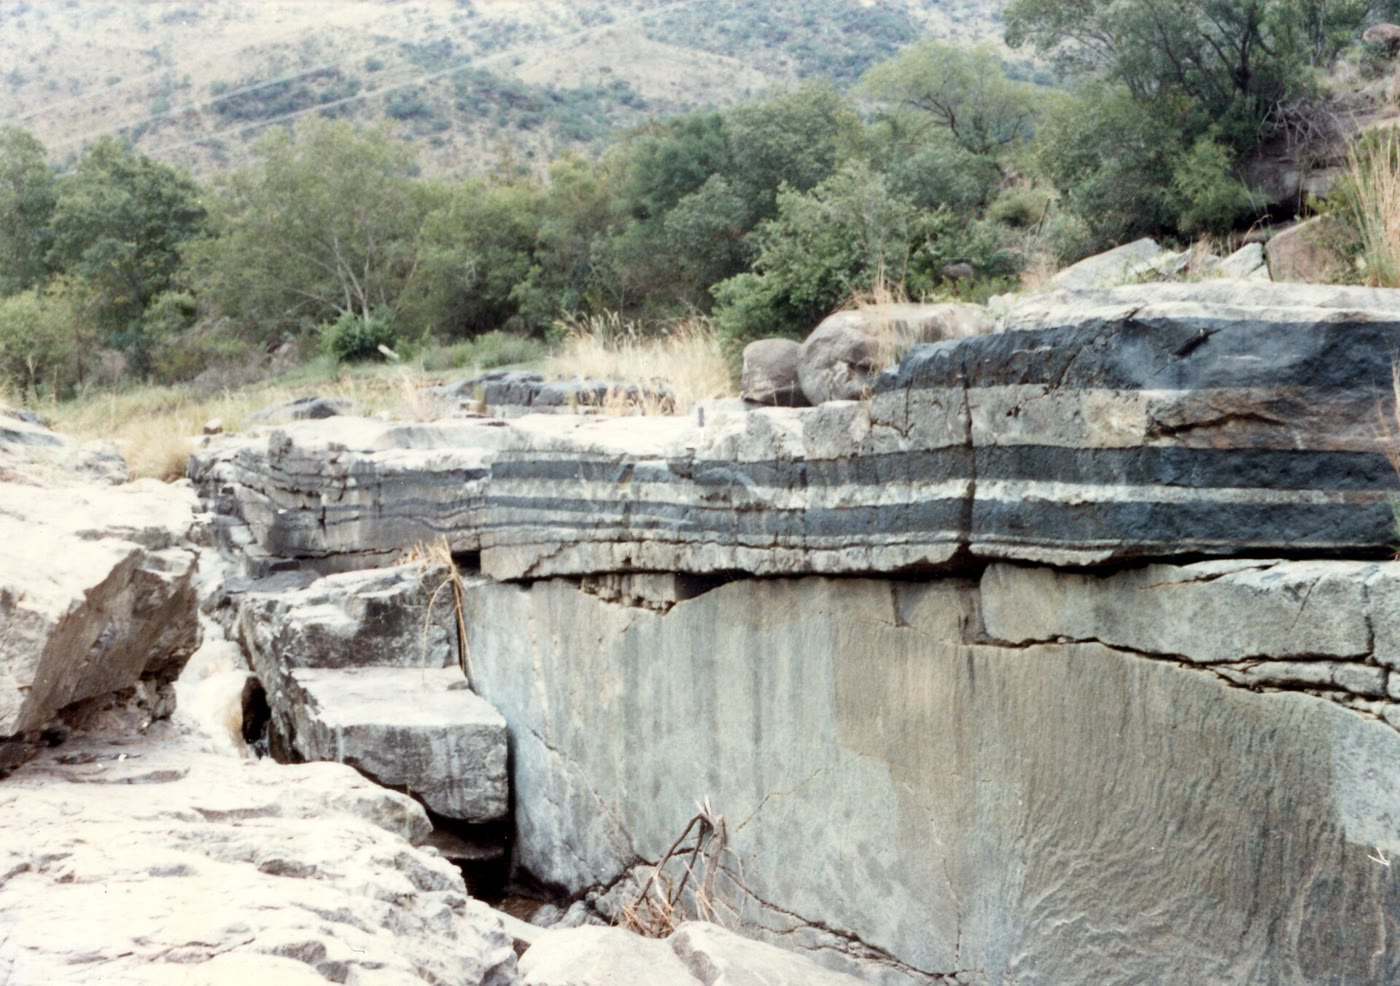
\includegraphics[height=5.2cm]{images/book4/b2-bushveld-chromitite.jpg}
\end{minipage}\hfill
\begin{minipage}[t]{0.42\linewidth}\vspace{0pt}\centering
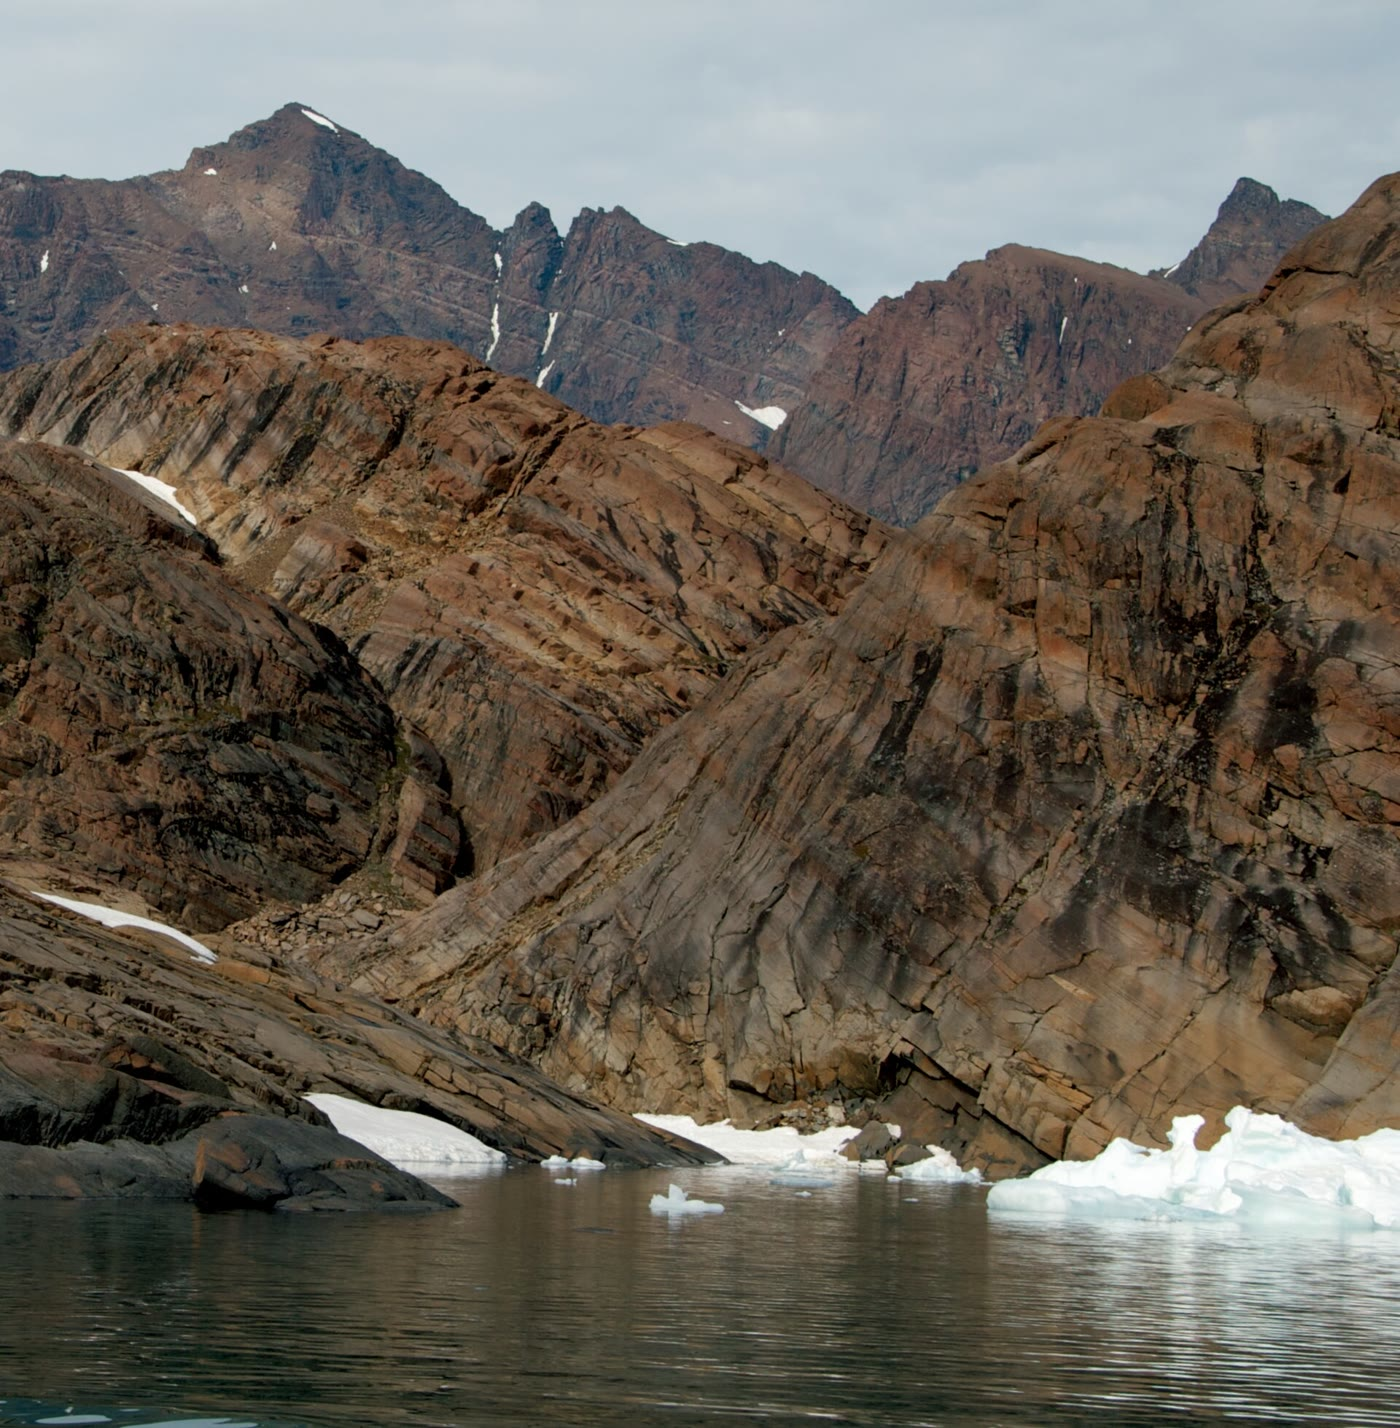
\includegraphics[height=5.2cm]{images/book4/b2-skaergaard-layering.jpg}
\end{minipage}
\par\smallskip{\small À esquerda: camadas de cromitito negro e de anortosito cinza da
Zona Crítica do Complexo de Bushveld, África do Sul (Kevin Walsh, CC BY 2.0).
À direita: os gabros acamados da Zona Média da intrusão de Skaergaard, leste da
Groenlândia, inclinados do alto à esquerda para baixo à direita (C. Tegner, CC BY 4.0).}
\end{omfigure}

\section{Sistemas abertos}\label{sec:b2:magmatic-differentiation:open}

Uma câmara magmática raramente é fechada. \omterm{def:b2:magma-emplacement:magma}{Magma} novo chega por baixo, e as paredes da
câmara são rochas que o \omterm{def:b2:magma-emplacement:magma}{magma} pode aquecer, fundir e dissolver.

\begin{definition}[Mistura de magmas; assimilação crustal; AFC]
\label{def:b2:magmatic-differentiation:open}
A \emph{mistura de magmas}\index{mistura de magmas} é a combinação de dois \omterm{def:b2:magma-emplacement:magma}{magmas} de composições
diferentes em um só. A \emph{assimilação crustal}\index{assimilação crustal} é a
incorporação de rocha crustal a um \omterm{def:b2:magma-emplacement:magma}{magma}, por fusão e dissolução da rocha das
paredes ou de blocos caídos nele. A \emph{assimilação--cristalização
fracionada}\index{assimilação--cristalização fracionada} (AFC) é sua
combinação em uma mesma câmara: o \omterm{def:b2:magma-emplacement:magma}{magma} cristaliza, e o calor latente liberado
funde e assimila a rocha das paredes.
\end{definition}

\begin{proposition}[A mistura é linear nas concentrações]\label{prop:b2:magmatic-differentiation:mixing}
Uma mistura de uma fração em massa $s$ do \omterm{def:b2:magma-emplacement:magma}{magma} A e $1-s$ do \omterm{def:b2:magma-emplacement:magma}{magma} B tem toda
concentração $C = sC_A + (1-s)C_B$: em qualquer diagrama de uma concentração em função de
outra, as misturas ficam sobre o segmento de reta de A a B, e a regra da alavanca dá
$s$.
\end{proposition}

\begin{proof}
Cada elemento se conserva: $C(m_A + m_B) = m_AC_A + m_BC_B$; divida-se por $m_A + m_B$.
\end{proof}

A mistura e a remoção de cristais traçam ambas retas nos \omterm{def:b2:magmatic-differentiation:harker}{diagramas de Harker}; as razões
isotópicas as distinguem. A cristalização não altera uma razão isotópica, ao passo que a
mistura com uma rocha de razão diferente a altera, ao longo da hipérbole do
\cref{ch:b2:isotope-geochemistry}. Um aumento de $^{87}$Sr/$^{86}$Sr com a sílica em uma
suíte vulcânica é portanto a marca da assimilação.

\begin{proposition}[Assimilação com cristalização fracionada]
\label{prop:b2:magmatic-differentiation:afc}
Um \omterm{def:b2:magma-emplacement:magma}{magma} cristaliza cristais de coeficiente de partição global $D$ para um elemento
e assimila rocha das paredes de concentração $C_a$ a uma taxa igual a $r$ vezes a taxa de
cristalização ($r \ne 1$). Sendo $F$ a massa de \omterm{def:b2:magma-emplacement:magma}{magma} relativa à sua massa
inicial e $z = (r + D - 1)/(r - 1)$,
\[
\frac{C}{C_0} = F^{-z} + \frac{r}{r - 1 + D}\,\frac{C_a}{C_0}\,\bigl(1 - F^{-z}\bigr).
\]
Para $r = 0$, esta é a lei de Rayleigh. A razão isotópica do elemento no \omterm{def:b2:magma-emplacement:magma}{magma}
é a média da do \omterm{def:b2:magma-emplacement:magma}{magma} inicial e da da rocha das paredes, ponderada pelos
dois termos desta soma.
\end{proposition}

\begin{proof}
Por unidade de massa inicial, quando uma massa $\mathrm dm_c$ cristaliza, uma massa
$r\,\mathrm dm_c$ é assimilada e a massa de \omterm{def:b2:magma-emplacement:magma}{magma} varia de $\mathrm dM =
-(1-r)\,\mathrm dm_c$. O balanço do elemento é $\mathrm d(MC) = rC_a\,\mathrm dm_c -
DC\,\mathrm dm_c$. Desenvolvendo o membro da esquerda e substituindo $\mathrm dm_c$ por
$-\mathrm dM/(1-r)$,
\[
M\frac{\mathrm dC}{\mathrm dM} = -C - \frac{rC_a - DC}{1-r}
= \frac{(r - 1 + D)\,C - rC_a}{1 - r} = -z\,\bigl(C - C^*\bigr),
\qquad C^* = \frac{rC_a}{r - 1 + D}.
\]
Assim, $\mathrm d(C - C^*)/(C - C^*) = -z\,\mathrm dM/M$, e $C - C^*$ é proporcional
a $M^{-z}$; com $C = C_0$ em $M = 1$, $C = C^* + (C_0 - C^*)F^{-z}$, que é a
fórmula. Para $r = 0$, $z = 1 - D$ e $C^* = 0$. Os átomos que vêm do
\omterm{def:b2:magma-emplacement:magma}{magma} inicial obedecem à mesma equação com $C_a = 0$, de modo que sua concentração é
$C_0F^{-z}$; o resto vem da parede: daí a ponderação das razões isotópicas.
\end{proof}

DePaolo deu essas equações em 1981, e elas são o modelo padrão de um \omterm{def:b2:magma-emplacement:magma}{magma}
contaminado em sua passagem pela crosta. Elas escondem uma restrição térmica. O calor
para assimilar rocha vem do calor latente dos cristais: aquecer crosta de
150 a \qty{1150}{\celsius} exige cerca de \qty{1}{kJ/g}, fundi-la \qty{300}{J/g},
enquanto o \omterm{def:b2:magma-emplacement:magma}{magma} que cristaliza fornece cerca de \qty{400}{J/g}; assim, uns \qty{3.25}{g} de
\omterm{def:b2:magma-emplacement:magma}{magma} precisam cristalizar para cada grama de rocha assimilada, e $r$ fica bem abaixo de 1.
Wilcox fez o mesmo cálculo para o Parícutin: seus \qty{25.4}{g} de quartzo-monzonito,
tomados a cerca de \qty{200}{\celsius}, precisavam de uns \qty{31350}{J} para serem
aquecidos a \qty{1100}{\celsius} e fundidos, o calor da cristalização de cerca de
\qty{85}{g} de plagioclásio, muito mais que os \qty{12.5}{g} de cristais que seu balanço
de massa removia. O \omterm{def:b2:magma-emplacement:magma}{magma} emitido não poderia ter pago sua própria assimilação:
o calor deve ter vindo de um corpo de \omterm{def:b2:magma-emplacement:magma}{magma} maior que aquele que entrou em erupção,
cristalizando longe da vista (\cref{exo:b2:magmatic-differentiation:11}).
% ledger: depaolo81:afc, white09:afc-heat, wilcox54:heat, wilcox54:mass-balance

\begin{omfigure}
\centering
\begin{tikzpicture}
\begin{axis}[omrecord, name=left, width=0.47\linewidth, height=5.4cm,
  xmin=0.3, xmax=1, ymin=0.3, ymax=1.05, x dir=reverse,
  xlabel={magma restante $F$}, ylabel={Sr: $C/C_0$},
  tick label style={font=\scriptsize}, label style={font=\small}]
\addplot[thick, black] table[x=F, y=srC_r0] {figdata/out/bachelor-2-differentiation-afc.dat};
\addplot[thick, blue!70!black] table[x=F, y=srC_r02] {figdata/out/bachelor-2-differentiation-afc.dat};
\addplot[thick, red!70!black] table[x=F, y=srC_r05] {figdata/out/bachelor-2-differentiation-afc.dat};
\end{axis}
\begin{axis}[omrecord, at={(left.east)}, anchor=west, xshift=1.7cm,
  width=0.47\linewidth, height=5.4cm,
  xmin=0.3, xmax=1, ymin=0.703, ymax=0.716, x dir=reverse,
  xlabel={magma restante $F$}, ylabel={$^{87}$Sr/$^{86}$Sr},
  y tick label style={/pgf/number format/fixed, /pgf/number format/precision=3},
  legend style={font=\scriptsize, at={(0.03,0.97)}, anchor=north west},
  tick label style={font=\scriptsize}, label style={font=\small}]
\addplot[thick, black] table[x=F, y=iso_r0] {figdata/out/bachelor-2-differentiation-afc.dat};
\addlegendentry{$r = 0$}
\addplot[thick, blue!70!black] table[x=F, y=iso_r02] {figdata/out/bachelor-2-differentiation-afc.dat};
\addlegendentry{$r = 0.2$}
\addplot[thick, red!70!black] table[x=F, y=iso_r05] {figdata/out/bachelor-2-differentiation-afc.dat};
\addlegendentry{$r = 0.5$}
\end{axis}
\end{tikzpicture}
\par\smallskip{\small Assimilação com \omterm{def:b2:magmatic-differentiation:crystallisation}{cristalização fracionada} para o estrôncio
($D = 1.5$, rocha das paredes com metade do estrôncio do \omterm{def:b2:magma-emplacement:magma}{magma} e
$^{87}$Sr/$^{86}$Sr = 0.7200, \omterm{def:b2:magma-emplacement:magma}{magma} 0.7035; valores ilustrativos). À esquerda: a
concentração cai mais depressa à medida que a taxa de assimilação $r$ aumenta, já que a rocha das paredes traz
menos estrôncio e mais cristais se formam para o mesmo $F$. À direita: a razão
isotópica, inalterada pela cristalização sozinha ($r = 0$), sobe em direção à da parede.}
\end{omfigure}

\section{Ler cristais zonados}\label{sec:b2:magmatic-differentiation:zoning}

\begin{definition}[Zonação composicional]\label{def:b2:magmatic-differentiation:zoning}
Um cristal de uma solução sólida apresenta \emph{zonação composicional}\index{zonação composicional}
quando sua composição varia do núcleo à borda, registrando o líquido em mudança
a partir do qual cresceram as camadas sucessivas. A zonação é \emph{normal} quando a borda é mais rica
no componente de baixa temperatura (o sódio no plagioclásio), \emph{inversa} quando é
mais rica no de alta temperatura, e \emph{oscilatória} quando alterna.
\end{definition}

Um cristal zonado é a \omterm{def:b2:magmatic-differentiation:crystallisation}{cristalização fracionada} apanhada em flagrante: seu núcleo não se
reequilibrou com o líquido posterior. A figura abaixo calcula, sobre o fuso de Bowen,
o plagioclásio que cresce a partir de um líquido com \qty{50}{\percent} de anortita. Em
equilíbrio, os cristais permanecem homogêneos e terminam com \qty{50}{\percent}; na \omterm{def:b2:magmatic-differentiation:crystallisation}{cristalização
fracionada} perfeita, cada nova camada está em equilíbrio com um líquido cada vez mais sódico,
e a borda dos últimos cristais é quase albita pura. A zonação normal, de
núcleo cálcico a borda sódica, é o que a série de Bowen prevê para um \omterm{def:b2:magma-emplacement:magma}{magma} que se resfria. Uma zona
inversa, uma faixa cálcica por fora de uma faixa sódica, diz que o cristal foi subitamente banhado por
um líquido mais quente ou mais cálcico: muitas vezes a chegada de \omterm{def:b2:magma-emplacement:magma}{magma} novo, a mistura na
câmara.
% ledger: bowen13:plagioclase, earle:bowen (Book 2)

\begin{omfigure}
\centering
\begin{tikzpicture}
\begin{axis}[omrecord, width=0.78\linewidth, height=6cm,
  xmin=0, xmax=1, ymin=0, ymax=90,
  xlabel={fração do líquido cristalizada},
  ylabel={anortita (\unit{\percent}, molar)},
  legend style={font=\scriptsize, at={(0.02,0.02)}, anchor=south west},
  tick label style={font=\scriptsize}, label style={font=\small}]
\addplot[very thick, red!70!black] table[x=x, y=an_frac] {figdata/out/bachelor-2-differentiation-zoning.dat};
\addlegendentry{fracionada: camada em formação}
\addplot[thick, gray, densely dotted] table[x=x, y=an_liq_frac] {figdata/out/bachelor-2-differentiation-zoning.dat};
\addlegendentry{fracionada: líquido}
\addplot[very thick, blue!70!black, dashed] table[x=x, y=an_eq] {figdata/out/bachelor-2-differentiation-zoning.dat};
\addlegendentry{equilíbrio: cristais}
\end{axis}
\end{tikzpicture}
\par\smallskip{\small Plagioclásio que cristaliza a partir de um líquido com \qty{50}{\percent}
de anortita, calculado sobre o fuso de Bowen (1913). Na \omterm{def:b2:magmatic-differentiation:crystallisation}{cristalização fracionada}, as
camadas sucessivas dos cristais, do núcleo (à esquerda) à borda (à direita), ficam cada vez mais
sódicas, e o líquido chega à albita quando cerca de \qty{82}{\percent} cristalizaram; na
\omterm{def:b2:magmatic-differentiation:crystallisation}{cristalização em equilíbrio}, os cristais permanecem uniformes e terminam com a composição do
líquido de onde vieram.}
\end{omfigure}

\begin{inthelab}[Ler cristais zonados]
Os petrólogos leem a zonação primeiro entre polarizadores cruzados, onde as zonas de um
plagioclásio se extinguem em ângulos ligeiramente diferentes e aparecem como faixas concêntricas.
Em seguida, eles a medem: uma microssonda eletrônica (\cref{ch:b2:field-lab-methods-2})
analisa pontos de alguns micrômetros ao longo de um perfil do núcleo à borda, e mapas
de cálcio e de sódio mostram as zonas diretamente. A partir de tal perfil, eles calculam a
composição do líquido a partir do qual cada zona cresceu, com o fuso da figura acima ou
com coeficientes de partição, e contam as zonas inversas como o número de
recargas da câmara. Os \omterm{def:b2:elements-in-the-earth:trace}{elementos-traço} medidos ao longo do mesmo perfil por ablação
a laser, e as razões isotópicas medidas zona por zona, separam cristalização, mistura
e assimilação na história de um único cristal.
\end{inthelab}

\section{Exercícios}

\begin{exercise}[$\star$]\label{exo:b2:magmatic-differentiation:1}
Use as medidas de Bowen sobre os plagioclásios (solidus / liquidus, \unit{\celsius}):
An$_{100}$ 1550 / 1550; An$_{83.3}$ 1465 / 1521; An$_{66.7}$ 1372 / 1490; An$_{50}$
1287 / 1450; An$_{33.3}$ 1205 / 1394; An$_{20}$ liquidus 1334; An$_{11.1}$ liquidus
1265, e interpole linearmente entre pontos vizinhos. Um líquido com
\qty{50}{\percent} de anortita se resfria em equilíbrio. (a) A que temperatura ele
começa a cristalizar, e qual é a composição do primeiro cristal? (b) A
\qty{1394}{\celsius}, quais são as composições do líquido e dos cristais,
e que fração em massa cristalizou (use as frações molares como se fossem frações
em massa)? (c) Qual é a composição da última gota de líquido?
\end{exercise}
% ledger: bowen13:plagioclase

\begin{exercise}[$\star$]\label{exo:b2:magmatic-differentiation:2}
Um \omterm{def:b2:magmatic-differentiation:cumulate}{cumulato} gabroico contém \qty{50}{\percent} de plagioclásio, \qty{35}{\percent} de
clinopiroxênio e \qty{15}{\percent} de olivina. Com os coeficientes de partição
(olivina / clinopiroxênio / plagioclásio) Sr 0.000063 / 0.157 / 2.7, Zr 0.00068 /
0.195 / 0.001 e Rb 0.000044 / 0.0033 / 0.025, calcule o coeficiente de partição
global de cada elemento, e diga qual é compatível.
\end{exercise}
% ledger: white07:kd-basalt

\begin{exercise}[$\star$]\label{exo:b2:magmatic-differentiation:3}
O \omterm{def:b2:magmatic-differentiation:cumulate}{cumulato} do \cref{exo:b2:magmatic-differentiation:2} cristaliza a partir de um basalto, por \omterm{def:b2:magmatic-differentiation:crystallisation}{cristalização fracionada},
até que reste metade do líquido. (a) Por que fator cada um de Sr, Zr e Rb variou
no líquido (tome os coeficientes globais 1.40, 0.069 e 0.014)? (b) Por que fator
a razão Zr/Rb variou? Comente com o corolário sobre as razões.
\end{exercise}
% ledger: white07:kd-basalt

\begin{exercise}[$\star$]\label{exo:b2:magmatic-differentiation:4}
A primeira lava do Parícutin (fevereiro de 1943) tinha \qty{55.04}{\percent} de \ce{SiO2},
\qty{5.68}{\percent} de \ce{MgO} e \qty{0.85}{\percent} de \ce{K2O}; a última (fevereiro de
1952), 60.07, 3.73 e \qty{1.67}{\percent}. (a) Calcule a variação de cada óxido.
(b) A potassa não entra em nenhum dos minerais que cristalizam. Se ela tivesse sido concentrada apenas
pela \omterm{def:b2:magmatic-differentiation:crystallisation}{cristalização fracionada}, que fração do líquido teria restado?
(c) O balanço de massa de Wilcox remove apenas cerca de \qty{12.5}{g} de cristais por
\qty{100}{g} de \omterm{def:b2:magma-emplacement:magma}{magma}. O que a comparação sugere?
\end{exercise}
% ledger: wilcox54:table2, wilcox54:mass-balance

\begin{exercise}[$\star\star$]\label{exo:b2:magmatic-differentiation:5}
Compare a \omterm{def:b2:magmatic-differentiation:crystallisation}{cristalização fracionada} e a \omterm{def:b2:magmatic-differentiation:crystallisation}{cristalização em equilíbrio}: calcule $C_L/C_0$ pelas duas leis
(a) para o níquel, $D = 5$, quando \qty{20}{\percent} do líquido cristalizou; (b)
para um \omterm{def:b2:elements-in-the-earth:partition}{elemento incompatível}, $D = 0.01$, quando \qty{90}{\percent} cristalizaram.
(c) Quais são os limites das duas leis quando $F \to 0$? Qual lei pode esgotar completamente um líquido de um
\omterm{def:b2:elements-in-the-earth:partition}{elemento compatível}?
\end{exercise}

\begin{exercise}[$\star\star$]\label{exo:b2:magmatic-differentiation:6}
(a) Calcule as porcentagens em massa de \ce{MgO}, \ce{FeO} e \ce{SiO2} na olivina
Fo$_{80}$, $(\ce{Mg}_{0.8}\ce{Fe}_{0.2})_2\ce{SiO4}$ ($M$ = 40.30, 71.84 e
\qty{60.08}{g/mol}). (b) Um basalto com \qty{10.0}{\percent} de \ce{MgO} e
\qty{49.0}{\percent} de \ce{SiO2} cristaliza apenas essa olivina até que seu líquido tenha
\qty{8.0}{\percent} de \ce{MgO}. Que fração em massa de olivina foi removida? (c) Qual
é então o teor de sílica do líquido?
\end{exercise}

\begin{exercise}[$\star\star$]\label{exo:b2:magmatic-differentiation:7}
Para a intrusão de Skaergaard, $F = \num{1.091e-7}H^2 - \num{5.9064e-4}H + 0.7678$.
(a) Calcule $F$ em $H = 0$, 1000 e \qty{2000}{m}. (b) A que altura $F = 0$?
(c) Que fração do \omterm{def:b2:magma-emplacement:magma}{magma} tinha cristalizado antes de se formar a base da sequência exposta do
assoalho, e onde ela poderia estar?
\end{exercise}
% ledger: tegner23:skaergaard

\begin{exercise}[$\star\star$]\label{exo:b2:magmatic-differentiation:8}
Ao longo da seção de Skaergaard, o \omterm{def:b2:magmatic-differentiation:cumulate}{cumulato} mediano contém \qty{177}{ppm} de Ni em
$F = 0.70$ (Zona Inferior a), \qty{54}{ppm} em $F = 0.29$ (Zona Média) e
\qty{6.2}{ppm} em $F = 0.17$ (Zona Superior a). (a) Supondo que os \omterm{def:b2:magmatic-differentiation:cumulate}{cumulatos} contêm
$D$ vezes o níquel de seu líquido e que o líquido segue a lei de Rayleigh,
calcule o $D$ aparente entre os dois primeiros níveis. (b) Faça o mesmo entre os
dois últimos. (c) O que pode fazer o $D$ aparente variar?
\end{exercise}
% ledger: data:b4-skaergaard

\begin{exercise}[$\star\star$]\label{exo:b2:magmatic-differentiation:9}
Verifique a resposta de Wilcox: \qty{100}{g} de matriz da primeira lava (\ce{SiO2}
55.53, \ce{MgO} 4.66, \ce{K2O} \qty{0.88}{\percent}) mais \qty{25.4}{g} de xenólito
médio (72.48, 0.77, 3.64) menos \qty{2.9}{g} de olivina Fo$_{80}$ (39.19, 42.06, 0)
menos \qty{9.6}{g} de plagioclásio An$_{70}$ (50.54, 0, 0). (a) Que massa resta?
(b) Calcule seus teores de \ce{SiO2}, \ce{MgO} e \ce{K2O} e compare com a matriz da
lava 19 (60.16, 3.19 e \qty{1.75}{\percent}). (c) Qual óxido se ajusta pior?
\end{exercise}
% ledger: wilcox54:groundmass, wilcox54:xenoliths, wilcox54:mass-balance

\begin{exercise}[$\star\star\star$]\label{exo:b2:magmatic-differentiation:10}
Um \omterm{def:b2:magma-emplacement:magma}{magma} assimila rocha das paredes a $r = 0.2$ enquanto cristaliza, com $D_{\ce{Sr}} =
1.5$, $C_a/C_0 = 0.5$, $^{87}$Sr/$^{86}$Sr inicial = 0.7035 e rocha das paredes 0.7200.
(a) Calcule $z$, $F^{-z}$ e $C/C_0$ em $F = 0.7$. (b) Compare com a \omterm{def:b2:magmatic-differentiation:crystallisation}{cristalização fracionada}
pura no mesmo $F$, e explique a diferença pela massa de cristais
formada em cada caso. (c) Calcule a $^{87}$Sr/$^{86}$Sr do \omterm{def:b2:magma-emplacement:magma}{magma}.
\end{exercise}

\begin{exercise}[$\star\star\star$]\label{exo:b2:magmatic-differentiation:11}
Siga o balanço térmico de Wilcox para o Parícutin. (a) Quanto calor um grama de quartzo-monzonito
precisa para ir de 200 a \qty{1100}{\celsius} (capacidade térmica
\qty{1.1}{J/(g.K)}) e depois fundir (\qty{250}{J/g})? (b) Quanto para
\qty{25.4}{g}? (c) Que massa de plagioclásio An$_{70}$ (calor latente \qty{370}{J/g})
precisa cristalizar para fornecê-lo? (d) Compare com os \qty{12.5}{g} de cristais do
balanço de massa, calcule a razão $r$ entre assimilação e cristalização, e diga o que
isso implica.
\end{exercise}
% ledger: wilcox54:heat, white09:afc-heat

\begin{exercise}[$\star\star\star$]\label{exo:b2:magmatic-differentiation:12}
Um basalto com \qty{250}{ppm} de Ni cristaliza primeiro só olivina ($D = 5$) até
$F = 0.8$, depois olivina com plagioclásio e clinopiroxênio (coeficiente global $D = 1.5$). (a)
Calcule o fator pelo qual o níquel varia em cada etapa, e o teor de níquel do
líquido em $F = 0.5$. (b) O que uma lei única com $D = 5$ teria previsto?
(c) Explique por que a lei de Rayleigh deve ser aplicada por etapas.
\end{exercise}

\section{Problema: a intrusão que escreveu sua própria história}

\begin{problem}[{Problema de fim de semana --- das camadas de um gabro à fração de
seu magma que ainda estava líquida no fim}]
\label{pb:b2:magmatic-differentiation:1}
Uma \omterm{def:b2:magma-emplacement:bodies}{soleira} de gabro acamado (inventada) cristalizou a partir de um basalto cuja \omterm{def:b2:magma-emplacement:aureole}{margem resfriada}
fornece a composição parental: \ce{SiO2} 49.5, \ce{Al2O3} 16.0, \ce{FeO} 10.0,
\ce{MgO} 9.0, \ce{CaO} 11.5, \ce{Na2O} 2.5, \ce{K2O} \qty{0.30}{\percent};
\qty{150}{ppm} de Ni e \qty{80}{ppm} de Zr. Os \omterm{def:b2:magmatic-differentiation:cumulate}{cumulatos} da zona inferior são formados de
\qty{20}{\percent} de olivina, \qty{50}{\percent} de plagioclásio e \qty{30}{\percent} de
clinopiroxênio; acima do nível em que a olivina desaparece, de \qty{55}{\percent} de
plagioclásio e \qty{45}{\percent} de clinopiroxênio. Tome os coeficientes de partição
(olivina / plagioclásio / clinopiroxênio) Ni 5.0 / 0 / 2.0 e Zr 0.0007 / 0.001 /
0.195. Composições dos minerais (\unit{\percent}): olivina \ce{MgO} 42.06, \ce{CaO} 0,
\ce{Al2O3} 0, \ce{SiO2} 39.19; plagioclásio 0, 14.36, 31.70, 50.54; clinopiroxênio
16.0, 20.5, 3.0, 51.5. Um \omterm{def:b2:magma-emplacement:bodies}{dique}
de rocha de granulação fina, alimentado pela câmara quando a camada mais alta cristalizou, tem
\ce{SiO2} 50.0, \ce{Al2O3} 14.1, \ce{FeO} 16.7, \ce{MgO} 4.9, \ce{CaO} 7.3,
\ce{Na2O} 3.4, \ce{K2O} \qty{0.75}{\percent} e \qty{188}{ppm} de Zr.

\noindent\textbf{Parte I --- Os coeficientes de partição das camadas.}
\begin{enumerate}
\item Calcule o coeficiente de partição global do níquel na zona inferior.
\item Calcule o do zircônio na zona inferior.
\item Calcule ambos na zona superior.
\item Qual elemento é compatível em cada zona? O níquel continua compatível quando
a olivina desaparece?
\item Que mineral contém a maior parte do zircônio dos \omterm{def:b2:magmatic-differentiation:cumulate}{cumulatos}, e por quê?
\item Por que fator Ni/Zr no líquido varia a cada redução de $F$ à metade na zona
inferior?
\end{enumerate}

\noindent\textbf{Parte II --- Curvas de Rayleigh ao longo da seção.}
\begin{enumerate}[resume]
\item Que teor de níquel você espera no \omterm{def:b2:magmatic-differentiation:cumulate}{cumulato} mais baixo, cristalizado em
$F = 1$?
\item Um \omterm{def:b2:magmatic-differentiation:cumulate}{cumulato} da zona inferior, mais acima, contém \qty{190}{ppm} de Ni. Em que $F$ ele
se formou?
\item Qual era então o teor de zircônio do líquido?
\item Nesse $F$, compare o níquel do líquido dado pelas leis fracionada e de
equilíbrio.
\item A olivina desaparece em $F = 0.55$. Calcule o teor de níquel do líquido
nesse ponto.
\item Calcule o níquel dos \omterm{def:b2:magmatic-differentiation:cumulate}{cumulatos} formados logo abaixo e logo acima desse
nível. Que feição um geólogo veria no perfil?
\item Calcule o níquel do líquido e do \omterm{def:b2:magmatic-differentiation:cumulate}{cumulato} em $F = 0.40$. Explique
a tendência.
\end{enumerate}

\noindent\textbf{Parte III --- O balanço de massa do último líquido.}
\begin{enumerate}[resume]
\item Escreva a equação de conservação do método para um óxido, com as massas
$x_{\mathrm{ol}}, x_{\mathrm{pl}}, x_{\mathrm{cpx}}$ removidas por \qty{100}{g} de
\omterm{def:b2:magma-emplacement:magma}{magma} parental e o \omterm{def:b2:magma-emplacement:bodies}{dique} como líquido derivado.
\item Escreva-a para \ce{MgO}, \ce{CaO} e \ce{Al2O3}.
\item Resolva o sistema $3 \times 3$.
\item Que fração do \omterm{def:b2:magma-emplacement:magma}{magma} parental resta como líquido?
\item Verifique a resposta com \ce{SiO2}: recalcule a sílica do líquido a partir das
massas encontradas.
\item Compare as proporções dos minerais removidos com as modas das duas
zonas.
\item A potassa não entra em nenhum dos minerais: que fração de líquido ela dá?
\end{enumerate}

\noindent\textbf{Parte IV --- A fração de líquido no topo.}
\begin{enumerate}[resume]
\item Por que fator o zircônio tinha aumentado no líquido quando a olivina desapareceu em
$F = 0.55$? Dê o teor de zircônio nesse momento.
\item A partir do zircônio do \omterm{def:b2:magma-emplacement:bodies}{dique}, calcule a fração de líquido restante quando
ele se formou, aplicando a lei da zona superior a partir de $F = 0.55$.
\item Refaça o cálculo com um $D = 0.07$ único desde o início. A resposta é
sensível aos detalhes de $D$?
\item O ferro subiu de 10.0 para \qty{16.7}{\percent} no líquido enquanto a sílica quase não
mudou. Que minerais são responsáveis, e que tipo de série magmática
isso prenuncia (\cref{ch:b2:magmatic-series})?
\item Os \omterm{def:b2:magmatic-differentiation:cumulate}{cumulatos} mais altos contêm \qty{47}{ppm} de Zr. Os cristais cúmulus sozinhos conteriam
$\bar D$ vezes o zircônio do líquido; que fração em massa de líquido aprisionado
(com a composição do \omterm{def:b2:magma-emplacement:bodies}{dique}) explica a análise?
\item Indique a fração do \omterm{def:b2:magma-emplacement:magma}{magma} original ainda líquida quando a camada mais alta
cristalizou, o número-chave deste problema, e compare as três estimativas
(elementos maiores, potassa, zircônio).
\end{enumerate}
\end{problem}
% ledger: white07:kd-basalt, matzen12:dni
